
\section{Solace PubSub+ Event Broker}
Solace PubSub+ ist ein Enterprise-Messaging-Broker, der als zentrales Vermittlungssystem in einer ereignisgesteuerten Architektur dient. Er ermöglicht die asynchrone Kommunikation zwischen verteilten Anwendungen über ein publish/subscribe-basiertes Paradigma. Nachfolgend werden Aufbau und Hauptmerkmale dieses Brokers erläutert – insbesondere die Nutzung von Topics und Queues, die Unterstützung des MQTT-Protokolls, Mechanismen zur Zugriffskontrolle (ACLs) sowie die Konfiguration über die SEMP-API. Abschließend erfolgt ein Vergleich mit anderen Messaging-Lösungen.

\subsection{Aufbau eines Message Brokers und Solace-Architektur}

Ein Message Broker wie Solace PubSub+ fungiert als Vermittler zwischen Sendern und Empfängern von Nachrichten. Publisher schicken Nachrichten an den Broker, welcher diese anhand von Metadaten (meist Topics) an interessierte Subscriber weiterleitet. Dadurch sind Publisher und Subscriber entkoppelt – weder muss der Publisher die Empfänger kennen, noch der Subscriber die Quelle der Nachricht \cite{Eugster2003}. Diese Entkopplung erhöht die Skalierbarkeit und Flexibilität des Systems erheblich. Der Broker übernimmt Verantwortung für das Routing, Filtering und ggf. Persistieren der Nachrichten.

Solace PubSub+ implementiert dieses Prinzip in einer \textit{Event Broker}-Architektur, die auf hohe Durchsatzraten und viele parallele Verbindungen ausgelegt ist. Eine Besonderheit von Solace ist die Unterstützung mehrerer Protokolle innerhalb desselben Brokers. So können Clients über unterschiedliche offene Standards wie AMQP 1.0, MQTT 3.1.1/5.0, REST (HTTP) oder JMS 1.1 mit dem Broker kommunizieren, ohne Gateway oder Übersetzer \cite{SolaceProtocols}. Diese Multi-Protokoll-Fähigkeit erlaubt z.B., dass IoT-Geräte via MQTT Daten publizieren, während Backend-Systeme dieselben Daten über JMS oder WebSockets abonnieren – der Broker überbrückt dabei transparent die Protokolle.

Intern organisiert Solace den Nachrichtenraum in sogenannten \textit{Message VPNs} (Virtual Private Networks). Ein Message VPN ist ein logisch isolierter Kontext innerhalb eines Brokers, der Mandanten-Trennung ermöglicht. Alle folgenden Objekte wie Topics, Queues, Clients und ac{acl}-Profile sind immer innerhalb eines bestimmten VPN definiert. Der Broker kann somit mehrere VPNs parallel betreiben, die wie separate virtuelle Broker fungieren.

Abbildung \ref{fig:broker-arch} zeigt schematisch die grundlegende Funktionsweise eines Pub/Sub-Brokers. Publisher senden Ereignisse an den Broker, der diese basierend auf Topic-Filtern an die verbundenen Subscriber verteilt. Solace unterscheidet hierbei zwei Qualitäten von Nachrichtenlieferung: zum einen flüchtige \textit{Direct Messages}, die nicht persistiert werden (QoS 0/1, “non-persistent”), zum anderen \textit{Guaranteed Messages}, die auf dem Broker gespeichert und bei Bedarf erneut zugestellt werden (QoS 1/2, “persistent”). Erstere bieten maximale Geschwindigkeit und werden nur an aktuell verbundene Empfänger zugestellt; Letztere werden in sogenannten \textit{Queues} vorgehalten, bis ein Empfänger sie abruft, wodurch keine Nachrichten verloren gehen \cite{SolaceDirectGuaranteed}. Durch diese Zweiteilung kann ein Event Broker sowohl hochvolumige Echtzeitdaten (z.B. Marktdaten-Feeds) effizient verteilen, als auch kritische Nachrichten zuverlässig zustellen, selbst wenn Empfänger vorübergehend offline sind.

\begin{figure}[h]
\centering
\begin{tikzpicture}[node distance=1.8cm, every node/.style={font=\small}]
  \node[draw, rounded corners, fill=blue!10, minimum width=2.5cm, minimum height=1cm] (broker) {Solace Broker};
  \node[left=4cm of broker, draw, fill=green!20, minimum width=2.2cm, minimum height=0.8cm] (pub1) {Publisher 1};
  \node[below=1.2cm of pub1, draw, fill=green!20, minimum width=2.2cm, minimum height=0.8cm] (pub2) {Publisher 2};
  \node[right=4.2cm of broker, draw, fill=orange!20, minimum width=2.5cm, minimum height=0.8cm] (sub1) {Subscriber 1};
  \node[below=1.2cm of sub1, draw, fill=orange!20, minimum width=2.5cm, minimum height=0.8cm] (sub2) {Subscriber 2 (Queue)};
  \node[above=1.0cm of broker, font=\small\bfseries] at (broker.north) {Topic: sensora/v1/send/controller123};

  \draw[->, thick] (pub1) -- node[above] {Publish} (broker);
  \draw[->, thick] (pub2) -- (broker);
  \draw[->, thick] (broker) -- node[above] {Subscribe (live)} (sub1);
  \draw[->, thick] (broker) -- node[below] {Persisted (Queue)} (sub2);
\end{tikzpicture}
\caption{Schematische Darstellung eines Publish/Subscribe Event Brokers mit Solace.}
\label{fig:broker-arch}
\end{figure}

\subsection{Topics und Queues in Solace PubSub+}

Solace PubSub+ verwendet ein hierarchisches Topic-System zur Adressierung von Nachrichten. Topics sind benannte Kanäle, die typischerweise durch mittels Schrägstrich / getrennte Hierarchieebenen strukturiert sind (z.B. Sensor/Temperatur/Aussen). Publisher veröffentlichen Nachrichten auf einem bestimmten Topic, und Subscriber können sich auf Topics (bzw. Muster davon) abonnieren. Eine Stärke von Solace ist, dass Topics \textit{dynamisch} und ohne Vorab-Konfiguration genutzt werden können – der Broker akzeptiert beliebige Topic-Strings und leitet Nachrichten entsprechend weiter. Für die Filterung unterstützen Topics Platzhalter: Das Zeichen * steht für genau ein Hierarchie-Level (ein Wort zwischen den Trennzeichen), während > als Wildcard für beliebig viele nachfolgende Hierarchieebenen fungiert. Beispielsweise würde ein Subscriber auf Topic Sensor/Temperatur/* alle Temperaturwerte aller Sensoren erhalten, während Sensor/> sämtliche Nachrichten im Topic-Pfad beginnend mit Sensor matcht. Diese flexiblen Wildcards erlauben eine inhaltliche Filterung der Ereignisse bereits auf Broker-Seite.

Neben der direkten Verteilung über Topics bietet Solace die Möglichkeit, Topics mit \textit{Queues} zu verknüpfen. Eine \textit{Queue} ist ein benannter, persistentierender Endpunkt auf dem Broker, der Nachrichten speichern kann. Queues dienen primär der Realisierung von Lastverteilung und Persistenz (Point-to-Point-Messaging): Subscriber können eine exklusive Verbindung zu einer Queue aufbauen und erhalten die dort gespeicherten Nachrichten in der Reihenfolge ihres Eingangs. Solace verknüpft nun das Topic- und Queue-Konzept dadurch, dass man einer Queue eine oder mehrere Topic-Abonnements geben kann. Die Queue fungiert damit als langlebiger Subscriber auf die entsprechenden Topics. Publiziert ein Publisher eine Nachricht auf einem solchen Topic mit persistenter Delivery-Mode (Persistent Message), so wird die Nachricht in der zugeordneten Queue abgelegt und steht dort zur Abholung bereit. Dieses Konzept erlaubt es, die Pub/Sub-Semantik mit der Zuverlässigkeit von Queues zu kombinieren. So kann man etwa erreichen, dass eine bestimmte Ereignisart (Topic) an mehrere unabhängige Dienste zugestellt wird, indem man pro Dienst eine eigene Queue mit demselben Topic-Subscription definiert – die Nachricht wird vom Broker dupliziert und landet in allen relevanten Queues (Fan-Out auf persistente Empfänger). Im Solace-System sind Queues standardmäßig langlebig und können Nachrichten auch über Broker-Neustarts hinweg speichern; optional können sie als \textit{exklusiv} (nur ein Verbraucher gleichzeitig) oder \textit{non-exklusiv} (mehrere konkurrierende Verbraucher) konfiguriert werden. \cite{SolaceTopicWildcard}.

Im Vergleich zu anderen Messaging-Brokern vereinheitlicht Solace damit das sonst oft getrennte Modell von Topics (für Pub/Sub) und Queues (für Punkt-zu-Punkt) zu einem flexiblen Konstrukt. Während z.B. in RabbitMQ Nachrichten immer an Exchanges gesendet und dann per Binding-Key auf Queues verteilt werden müssen, kann in Solace direkt auf einem Topic publiziert werden, das entweder von Clients abonniert oder von Queues “belauscht” wird \cite{SolaceTopicWildcard}. Auch JMS unterscheidet zwischen Topic und Queue als verschiedenen Destination-Typen; Solace als JMS-Provider mappt jedoch JMS-Topics und -Queues intern auf das gleiche einheitliche Event-Model, was Verwaltung und Integration erleichtert.

\subsection{MQTT und topic-basiertes Routing}

Das \textit{Message Queuing Telemetry Transport} (MQTT) Protokoll ist ein offener Standard für Leichtgewichts-Messaging, der vor allem im IoT-Umfeld verbreitet ist. Solace PubSub+ unterstützt MQTT in den Versionen 3.1.1 und 5.0 gemäß dem OASIS-Standard \cite{SolaceMQTT}. MQTT-Clients können sich mit dem Broker verbinden und Nachrichten auf MQTT-Topics publizieren bzw. abonnieren. Ein wesentliches Konzept von MQTT ist das topic-basierte Routing – analog zum oben beschriebenen Topic-System. MQTT-Themenpfade sind ebenfalls hierarchisch mit / aufgebaut; als Wildcards dienen "+" (ein Level) und "\#"(mehrere Level). Solace setzt diese MQTT-Semantik um und übersetzt sie intern auf das eigene Topic-Format. Beispielsweise entspricht ein MQTT-Subscription auf \code{\url{sensors/+/humidity}} einem Solace-Topicfilter \code{sensors/*/humidity}. Dadurch können MQTT-Publisher und -Subscriber nahtlos mit anderen Solace-Clients interagieren. So ist es möglich, dass ein Gerät via MQTT auf \code{sensors/room1/humidity} sendet, während ein Java-Anwendung über JMS das Topic \code{sensors/>} abonniert und somit die Nachricht erhält – der Broker übernimmt die Protokollkonvertierung und das Routing \cite{SolaceProtocols}.

MQTT sieht per Spezifikation keine expliziten Queues vor; wenn ein MQTT-Subscriber offline geht (und QoS 1 oder 2 verwendet), puffert der Broker die Nachrichten in einer Session-Queue, die beim Wiederverbinden ausgeliefert werden. Solace erweitert diese Möglichkeiten insofern, als dass man persistente Weiterleitung an benannte Queues nutzen kann, indem man MQTT-Themen mit Solace-Queues verknüpft (wie zuvor beschrieben). Rein mit MQTT-Mitteln kann ein Device also nur mittels Durable Session (Clean Session = false) Nachrichten nachliefern lassen, während Solace auch langfristige Persistenz über MQTT hinaus bietet. Allerdings gelten Protokolleinschränkungen: z.B. unterstützt MQTT v3.1.1 keine Bearbeitung von auf einer Queue gespeicherten Nachrichten, da das Konzept im Protokoll fehlt. Daher wird in Szenarien mit Bedarf an fortgeschrittenem Queueing ggf. ein anderes Protokoll (AMQP 1.0 oder Solaces eigenes API/SMF) verwendet \cite{SolaceDaprMQTT}. Nichtsdestotrotz unterstreicht die MQTT-Fähigkeit von Solace die Flexibilität des Brokers, heterogene Clients in ein gemeinsames Topic-basiertes Kommunikationsgeflecht einzubinden.

\subsection{Access Control Lists (ACLs)}

In einem Multi-User-Messaging-System ist feingranulares Zugriffsmanagement essenziell, um Sicherheit und Mandantentrennung zu gewährleisten. Solace PubSub+ bietet hierzu \textit{Access Control List (ACL) Profiles} an, mit denen reguliert wird, welche Aktionen ein Client ausführen darf. Ein ac{acl}-Profil bestimmt erstens, ob sich ein Client überhaupt mit dem Broker/Message-VPN verbinden darf, und zweitens, welche Topics er publizieren oder abonnieren darf \cite{SolaceACL}. Konkret bestehen ac{acl}-Profile aus Regeln, die Verbindungsversuche sowie Topic-Zugriffe kontrollieren. Für jede dieser Kategorien (Connect, Publish-Topic, Subscribe-Topic, sowie Subscribe auf Shared-Queues) lässt sich ein Standardverhalten definieren – entweder \textit{allow} (erlauben) oder \textit{deny} (standardmäßig verweigern) – und es können Ausnahmeregeln (\textit{exceptions}) für spezifische Topics oder Topic-Muster hinzugefügt werden.

Jedem Client, der sich authentifiziert, wird ein ac{acl}-Profil zugewiesen (entweder direkt am Client-Username konfiguriert oder – falls LDAP-Authentifizierung genutzt wird – über Gruppenzuordnung). Nach erfolgreicher Authentisierung prüft der Broker sämtliche Aktionen des Clients gegen die ac{acl} des zugewiesenen Profils. Beispielsweise kann ein ac{acl}-Profil erlauben, dass der Client nur auf Topics unterhalb von ClientA/> publizieren darf und alle anderen Topics geblockt werden. Versucht der Client eine Nachricht auf ein nicht erlaubtes Topic zu senden oder eine unberechtigte Subscription anzulegen, verweigert der Broker die Operation. Auf diese Weise können unterschiedliche Clients auf unterschiedliche Topic-Räume beschränkt werden, was im IoT-Umfeld z.B. dazu genutzt wird, dass jedes Gerät nur auf seinem eigenen Topic-Präfix senden/empfangen darf \cite{AvnetPSK}. ac{acl}-Profile sind damit ein zentrales Sicherheitsmerkmal, um unerlaubten Datenzugriff zu verhindern und eine saubere Mandantentrennung innerhalb eines Brokers (bspw. zwischen verschiedenen Anwendungen im selben Message VPN) sicherzustellen.

\subsection{Konfiguration über die SEMP-API}

Die Administration eines Solace-Brokers kann neben grafischen Tools und dem CLI auch vollständig automatisiert über eine REST-basierte Managementschnittstelle erfolgen – die \textit{Solace Element Management Protocol} API in Version 2 (\textbf{SEMP v2}). SEMP v2 stellt eine REST/HTTP-JSON API bereit, mit der sich der Broker programmatisch konfigurieren und überwachen lässt \cite{SolaceSEMP}. Über definierte Endpunkte können Management-Clients z.B. Queues oder Topic-Endpunkte anlegen, ac{acl}-Profile definieren, den Status von Clients und VPNs abfragen oder Verwaltungsaktionen (wie das Leeren einer Queue) durchführen. Die SEMP-API ist in drei Bereiche gegliedert: \begin{itemize}\setlength\itemsep{0pt} \item \textbf{Config}: Änderung und Abfrage der Konfigurationsobjekte \\(z.B. \verb|POST /SEMP/v2/config/msgVpns/{vpn}/queues| zum Anlegen einer Queue). \item \textbf{Monitor}: Lesezugriff auf betrieblichen Status und Metriken (z.B. Statistiken einer Queue, Anzahl der Clients etc.). \item \textbf{Action}: Auslösen von Aktionen, die keinen dauerhaften Konfigurationszustand ändern (z.B. \textit{Purge} einer Queue, Failover umschalten). \end{itemize} SEMP v2 ist via OpenAPI-Spezifikation beschrieben und ermöglicht so die automatisierte Generierung von Client-Bibliotheken \cite{SolaceSEMP}. In der Praxis kann somit z.B. ein Auth-Service mittels SEMP beim Deployment sicherstellen, dass benötigte Topics, Queues und ac{acl}s im Broker eingerichtet sind, ohne manuell die Admin-Oberfläche bedienen zu müssen. Die Verwendung einer Management-API erleichtert die Integration des Brokers in Infrastructure-as-Code und DevOps-Prozesse. Insbesondere in Cloud-Umgebungen mit dynamischer Skalierung kann der Broker so automatisiert auf neue Services oder geänderte Sicherheitsrichtlinien konfiguriert werden.

\subsection{Vergleich mit anderen Messaging-Systemen}
Solace PubSub+ steht in Konkurrenz zu einer Reihe von Messaging-Systemen, die teils unterschiedliche Architekturen aufweisen. Im Folgenden werden einige charakteristische Unterschiede kurz herausgestellt:
\textbf{RabbitMQ}: RabbitMQ ist ein verbreiteter Open-Source Message Broker, der das AMQP 0.9.1 Protokoll verwendet. Ähnlich wie Solace unterstützt RabbitMQ Publish/Subscribe und Queueing, jedoch meist nur über AMQP (Multi-Protokoll-Fähigkeit ist bei RabbitMQ nur über Plugins begrenzt möglich). RabbitMQ nutzt ein Exchange-Queue-Modell: Publisher senden an Exchanges, welche die Nachrichten anhand von Routing-Keys an Queues binden. Solace hingegen erlaubt das direkte Publizieren auf Topics, die intern sowohl von Abonnements als auch von Queues “gelesen” werden können \cite{SolaceTopicWildcard}. In Solace ist somit das Routing-Konzept etwas einfacher, da kein separater Exchange-Schritt sichtbar ist. Bezüglich Performance skaliert Solace durch seine optimierte Architektur und optional spezialisierte Hardware-Appliances auf sehr hohe Durchsätze, während RabbitMQ für viele Anwendungsfälle ausreichend, aber in extremen Szenarien früher an Grenzen stoßen kann. RabbitMQ bietet dafür eine große Flexibilität durch Plugins (etwa für unterschiedliche Auth-Backends, Shovel/Federation für verteilte Setups usw.), wohingegen Solace viele Funktionen nativ integriert (etwa eingebaute Hochverfügbarkeit, Replay-Funktionalität, etc.).
\textbf{Apache Kafka}: Kafka verfolgt einen anderen Ansatz als klassische Message Broker. Es ist eigentlich eine verteilte Commit-Log-Plattform, die primär für Streaming von Datenströmen und Event Sourcing konzipiert ist. Im Gegensatz zu Solace, das Nachrichten direkt an Subscriber weiterleitet oder zwischenpuffert, schreibt Kafka alle Nachrichten fortlaufend in Partitionen auf Disk. Consumer lesen diese logischen Partitionen in eigenem Tempo und behalten Zustände wie den Lese-Offset. Dadurch eignet sich Kafka hervorragend für das Replaying vergangener Events und das Verteilen großer Datenmengen auf viele Konsumenten, hat aber keinen Broker, der aktiv zu Clients zustellt – die Clients holen vielmehr die Daten. Solace dagegen ist auf Live-Zustellung optimiert: Nachrichten werden typischerweise verworfen, wenn kein Abnehmer da ist (außer es existiert eine persistente Queue). Man könnte vereinfacht sagen, Kafka speichert Streams dauerhaft (Standard ist Tage bis unbegrenzt) und garantiert dadurch Zustellung an spätere Konsumenten, während Solace klassischere Messaging-Semantiken bietet, wo persistente Nachrichten gezielt zugestellt und nach Bestätigung gelöscht werden (ähnlich JMS). Für use-cases im Auth-Service-Umfeld (kurzlebige Ereignisse, Befehle, Responses) ist ein Broker wie Solace passender; Kafka spielt seine Stärken bei Analyse- und Loggingdaten aus \cite{Kreps2011}.
\textbf{JMS Broker (ActiveMQ/IBM MQ) und Andere}: Solace kann auch als JMS-Provider dienen und vergleichbare Funktionalität wie ActiveMQ, Artemis oder IBM MQ bereitstellen. Gegenüber vielen JMS-Brokern punktet Solace mit integrierter Mehrprotokollfähigkeit und höherer Performance. IBM MQ etwa ist stark auf Transaktionssicherheit und Mainframe-Integration ausgelegt, während Solace auf niedrige Latenz und flexible Verteilung optimiert ist. Moderne Cloud-Messaging-Services (AWS SNS/SQS, Azure Service Bus) trennen oft Pub/Sub und Queuing in separate Services – Solace bietet beides in einem. Insgesamt ist Solace als \glqq Enterprise Event Broker\grqq{} positioniert, der in verteilten Architekturen (z.B. Microservices, IoT, Hybrid-Cloud) eine zentrale Kommunikationsdrehscheibe bildet und durch Features wie \textit{Dynamic Message Routing} (für geclusterte Broker-Netze, Event Mesh) und eingebaute Hochverfügbarkeit auszeichnet.
Zusammenfassend lässt sich festhalten, dass Solace PubSub+ aufgrund seines architektonischen Designs (vereinheitlichtes Topic/Queue-Model, Multi-Protokoll-Unterstützung, hohe Performance) eine besondere Rolle unter den Messaging-Systemen einnimmt. Die theoretischen Grundlagen dieses Brokers – Entkopplung durch Pub/Sub, Hierarchie-Topics, etc. – bilden die Basis für den praktischen Einsatz im Rahmen des Auth-Service, wo Solace die Nachrichtenkommunikation absichert und steuert.


\section{Sicherheitsrelevante Technologien im Auth-Service}

Im Auth-Service kommen mehrere kryptographische und sicherheitstechnische Verfahren zum Einsatz, um die Authentifizierung und Kommunikation abzusichern. In diesem Abschnitt werden die folgenden Konzepte erläutert:
\textbf{HMAC} (Hash-based Message Authentication Code) – ein Verfahren zur Gewährleistung von Nachrichtenintegrität und -authentizität.
\textbf{Fernet-Verschlüsselung} – ein symmetrisches Authenticated-Encryption-Schema zur sicheren Ausgabe von Tokens.
\textbf{Tokenisierung mit PSK und Challenge-Response} – das Zusammenspiel von vorab geteilten Schlüsseln (Pre-Shared Keys), Challenge-Response-Authentifizierung und der Verwendung von Tokens im Authentifizierungsprozess.
Ziel ist es, die kryptographischen Grundlagen, Funktionsweisen und Sicherheitseigenschaften dieser Techniken darzustellen, um das Verständnis für ihre Umsetzung im Auth-Service zu schaffen.

\subsection{HMAC: Hash-basierter Message Authentication Code}

Ein \textit{Message Authentication Code} (MAC) ist eine Prüfsumme, die unter Verwendung eines geheimen Schlüssels berechnet wird und es Empfängern ermöglicht, die Integrität und Authentizität einer Nachricht zu verifizieren. Der Sender berechnet einen MAC-Wert über die Nachricht und sendet ihn mit; der Empfänger kann mit dem geteilten Geheimnis denselben MAC berechnen und vergleichen. Stimmen die Werte überein, ist sichergestellt, dass die Nachricht unverändert ist und vom legitimen Sender stammt (solange der Schlüssel geheim bleibt).

HMAC (\textit{Keyed-Hash Message Authentication Code}) ist ein spezielles, sehr weit verbreitetes MAC-Verfahren, das auf kryptographischen Hashfunktionen basiert \cite{RFC2104}. Formal lässt sich HMAC definieren als: 

$\mathbf{HMAC_{k}}(m)=H((K⊕opad)∥H((K⊕ipad)∥m))$, wobei $H$ eine kryptographische Hashfunktion (etwa SHA-256) und $K$ ein geheimer Schlüssel ist (typischerweise auf Blockgröße von $H$ aufgefüllt). Die Konstanten $opad$ und $ipad$ sind bitmasken (\textit{outer/inner padding}), die den Schlüssel vor dem Hashen modifizieren. Durch diese zweistufige Konstruktion (Hash innerhalb eines Hashs) werden bestimmte Angriffe auf einfachere MAC-Konstruktionen (wie \glqq Schlüssel+Nachricht hashen\grqq) verhindert. Intuitiv berechnet HMAC zunächst einen Hash der Kombination aus Schlüssel und Nachricht und hasht dieses Ergebnis nochmals zusammen mit dem Schlüssel.

HMAC wurde 1996 von Bellare, Canetti und Krawczyk entwickelt und analysiert. In RFC 2104 ist HMAC als generisches Konstrukt spezifiziert, das mit jeder iterativen Hashfunktion (MD5, SHA-1, SHA-2 etc.) genutzt werden kann \cite{RFC2104}. So verwendet HMAC-SHA256 beispielsweise die Secure Hash Algorithm 256-bit Funktion als $H$. Die Sicherheit von HMAC hängt von den Eigenschaften der zugrundeliegenden Hashfunktion ab, insbesondere deren Kollisionsresistenz und Unberechenbarkeit \cite{RFC2104}. Unter typischen Annahmen lässt sich zeigen, dass HMAC annähernd ein \textit{pseudorandom function (PRF)} ist, solange $H$ keine gravierenden Schwächen aufweist – informell bedeutet dies, dass ohne Kenntnis des Schlüssels kein effizienter Weg bekannt ist, um den korrekten MAC für eine neue Nachricht zu erzeugen oder eine gültige Nachricht+MAC zu modifizieren. HMAC ist zudem resistent gegen sogenannte \textit{Längenextensierungs-Angriffe}, die bei einfachen Hash-MACs auftreten könnten, weil durch die Verwendung von $opad$/$ipad$ die innere Struktur des Hashs gesichert wird.

Aufgrund seiner starken Sicherheitseigenschaften und Einfachheit ist HMAC in vielen Protokollen und Standards fest verankert. Das US-amerikanische NIST standardisierte HMAC in FIPS 198-1 \cite{FIPS198}. In TLS und IPsec dient HMAC (mit SHA-256 oder SHA-384) als Nachrichten-Authentifizierungsmechanismus, um die Integrität von übertragenen Daten sicherzustellen. Auch viele Anwendungsschichten nutzen HMAC: Beispielsweise beruht der HOTP-Algorithmus (HMAC-based One-Time Password) für Einmalpasswörter auf einem HMAC über einen Zähler \cite{RFC4226}, und JSON Web Tokens (JWT) können mit einem HMAC-SHA256 (\texttt{HS256}) Signaturteil versehen sein, um Tokenintegrität zu gewährleisten.

Im Kontext des Auth-Service wird HMAC insbesondere im Rahmen eines \textit{Challenge-Response}-Verfahrens eingesetzt. Hierbei teilen sich der Client (z.B. ein IoT-Gerät) und der Server einen geheimen Schlüssel $K$ (siehe \glqq Pre-Shared Key\grqq{} unten). Zur Authentifizierung sendet der Server dem Client eine Zufallsherausforderung (Nonce) – typischerweise eine ausreichend lange zufällige Bitfolge $N$. Der Client berechnet daraufhin den HMAC-Wert über diese Challenge:
R=HMACk(N). Dieser Response-Wert $R$ wird an den Server zurückgesendet. Da der Server ebenfalls $K$ kennt, kann er seinerseits $\mathrm{HMAC}_K(N)$ berechnen und prüfen, ob das Ergebnis mit dem empfangenen $R$ übereinstimmt. Ist dies der Fall, beweist der Client damit, dass er den geheimen Schlüssel besitzt (denn nur mit $K$ lässt sich der korrekte MAC erzeugen). Gleichzeitig wird die Integrität der Challenge gewährleistet – eine Manipulation von $N$ unterwegs würde zu einem falschen MAC führen. Wichtig ist, dass für jede neue Authentifizierung eine frische, unvorhersehbare Challenge $N$ gewählt wird, um Wiederholungsangriffe (Replay) zu verhindern. Dieses einfache Challenge-Response-Schema bietet eine zuverlässige Einweg-Authentifizierung des Clients gegenüber dem Server, ohne dass der Schlüssel selbst jemals übertragen wird. Die Verwendung von HMAC dafür ist ideal, da HMAC effizient berechenbar ist (auch auf eingeschränkter Hardware) und kryptographisch stark genug, um nicht geraten oder invertiert werden zu können.

Zusammengefasst liefert HMAC also einen grundlegenden Baustein für die Nachrichtenauthentifizierung: mathematisch basiert es auf Hashfunktionen und verknüpft einen geheimen Schlüssel mit der Nachricht zu einem Prüftoken. Seine Sicherheit wurde analytisch untermauert \cite{Krawczyk1997} und in Praxisstandards übernommen, was es zu einem vertrauenswürdigen Mechanismus für Integritätsschutz macht. Im Auth-Service bildet HMAC den Kern des Authentifizierungsnachweises im Challenge-Response-Protokoll.


\subsection{Fernet-Verschlüsselung: Authenticated Encryption für Tokens}

Neben der Überprüfung von Nachrichtenintegrität (via MAC) ist oft auch Vertraulichkeit und Schutz vor Manipulation bei gespeicherten oder übertragenen Tokens erforderlich. \textit{Fernet} ist ein hochrangiges kryptographisches Schema, das symmetrische Verschlüsselung mit Integritätsschutz kombiniert und dadurch sog. \textit{Authenticated Encryption} bereitstellt. Es wurde ursprünglich als Teil der Python-Kryptographiebibliothek entwickelt, liegt aber als offene Spezifikation vor und ist in mehreren Sprachen implementiert \cite{cryptographyFernet}. Fernet garantiert, dass ein verschlüsselter Datenträger (Token) weder gelesen noch unbemerkt verändert werden kann, ohne den geheimen Schlüssel zu besitzen \cite{cryptographyFernet}.

Technisch basiert Fernet auf anerkannten Standard-Primitiven: \begin{itemize}\setlength\itemsep{0pt} \item \textbf{Verschlüsselung}: AES im CBC-Modus mit 128-Bit-Schlüssel und PKCS\#7 Padding wird verwendet, um die eigentlichen Nutzdaten zu chiffrieren. \item \textbf{Integrität/Authentizität}: Ein HMAC über die verschlüsselten Daten (inkl. Header) mit SHA-256 stellt sicher, dass Änderungen erkannt werden. \item \textbf{Zufall}: Für jede Verschlüsselung wird ein frischer 128-Bit Initialisierungsvektor (IV) per Kryptozufall erzeugt. \end{itemize} Diese Details sind in der Fernet-Spezifikation festgelegt \cite{FernetSpec}. Ein Fernet-Schlüssel ist 32 Byte (256 Bit) lang und wird intern in zwei Hälften aufgeteilt: 16 Byte dienen als AES-Schlüssel, 16 Byte als HMAC-Schlüssel \cite{FernetSpec}. Bei der Token-Erstellung wird folgendermaßen verfahren \cite{FernetSpec}:
\begin{enumerate}
    \item Es wird ein 64-Bit-Zeitstempel (Sekunden seit Unix-Epoche) als \textit{Timestamp} festgehalten, der den Erstellungszeitpunkt markiert.
    \item Ein zufälliger 16-Byte IV wird generiert.
    \item Die Klartextnachricht wird mit AES-128-CBC unter Verwendung des IV und des Verschlüsselungsschlüssels verschlüsselt (nachdem sie mit PKCS7 auf Blocklänge aufgefüllt wurde).
    \item Über den sogenannten Token-Header (bestehend aus einer 8-Bit Versionskennung, dem Timestamp und dem IV) \textit{und} den Ciphertext wird ein HMAC-SHA256 mit dem HMAC-Schlüssel berechnet
    \item  Der finale Fernet-Token besteht aus der Konkatenation von Version, Timestamp, IV, Ciphertext und HMAC. Dieser Byte-String wird zuletzt URL-sicher Base64-kodiert, um ihn als ASCII-Token darstellbar zu machen. Das Format eines Fernet-Tokens lässt sich schematisch so darstellen: 


\[
\underbrace{\texttt{0x80}}_{\text{Version}} 
\quad
\underbrace{T_{\text{stamp}}}_{\text{64-Bit-Zeit}} 
\quad
\underbrace{IV}_{\text{128-Bit}} 
\quad
\underbrace{C}_{\text{Ciphertext}} 
\quad
\underbrace{\mathrm{HMAC}}_{\text{256-Bit}},
\]
,wobei $C$ variable Länge (Vielfaches von 128 Bit) hat, abhängig von der Klartextlänge \cite{FernetSpec}. Die Versionsnummer ist aktuell immer 0x80 (Version 1 der Spezifikation). Der HMAC deckt den gesamten Token ohne das HMAC-Feld ab, d.h. $HMAC = \mathrm{HMAC}{K{\text{HMAC}}}(\text{Version} \parallel T_{\text{Stamp}} \parallel IV \parallel C)$ \cite{FernetSpec}. Dadurch wird sichergestellt, dass sowohl Header als auch Ciphertext geschützt sind – eine Veränderung irgendeines Bits im Token führt zu einem HMAC-Mismatch beim Entschlüsseln.
\end{enumerate}

Fernet ist somit ein klar strukturierter Fall von \textit{Encrypt-then-MAC}: Zuerst werden Daten symmetrisch verschlüsselt, dann wird über das Chiffrat ein MAC gebildet. Diese Konstruktion gilt als sicher (im Sinne von IND-CCA2, also Wahrung von Vertraulichkeit auch gegen adaptive Angreifer), da ein Empfänger immer erst den MAC prüft, bevor er entschlüsselt. Ohne Kenntnis des Schlüssels kann ein Angreifer weder den Ciphertext sinnvoll entschlüsseln noch einen gültigen neuen Token erzeugen, da ihm sowohl der AES- als auch der MAC-Schlüssel fehlen.

Die Verwendung von Standardbausteinen (AES, HMAC) stellt sicher, dass Fernet auf bekannten Sicherheitsannahmen beruht. AES-128 ist ein symmetrischer Blockcipher, der als praktisch sicher gilt; CBC-Modus ist sicher, solange jedes IV nur einmalig verwendet wird (was durch die zufällige Wahl gegeben ist). HMAC-SHA256 ist, wie oben erläutert, ein starker MAC. Die Kombination ergibt einen symmetrischen Authenticated-Encryption-Algorithmus, der konzeptionell ähnlich ist zu anderen AEADs (Authenticated Encryption with Associated Data) wie AES-GCM – allerdings mit dem Unterschied, dass Fernet die Komponenten explizit trennt und kein zusätzliches Associated Data Feature hat. Ein Vorteil von Fernet ist die Einfachheit der Schnittstelle: Entwickler erhalten eine einzige Routine zum Verschlüsseln und Entschlüsseln von Bytestrings, wodurch Implementierungsfehler (wie Vergessen der MAC-Prüfung oder unsichere IV-Wahl) vermieden werden. Die Fernet-Implementierung in der Python-\texttt{cryptography}-Bibliothek z.B. stellt sicher, dass bei Aufruf von decrypt(token) automatisch der HMAC geprüft und bei Scheitern eine Exception geworfen wird, sodass kein Entwickler versehentlich mit unverifizierten Daten weiterarbeitet \cite{cryptographyFernet}.

Für den Auth-Service ist besonders relevant, dass Fernet-Tokens einen eingebetteten Zeitstempel besitzen. Dies erlaubt es, die Gültigkeit von Tokens zeitlich zu begrenzen: Beim Entschlüsseln kann der Server den im Token codierten Erstellungszeitpunkt mit der aktuellen Zeit vergleichen und ein Token ggf. als abgelaufen verwerfen, wenn es älter als eine definierte TTL (time-to-live) ist. Somit kann ein vom Auth-Service ausgestelltes Token z.B. nur für eine Stunde gültig sein, danach muss sich der Client neu authentifizieren. Fernet selbst erzwingt keine Ablaufprüfung, bietet aber die Information (Timestamp) dafür an.

Ein weiteres Merkmal ist die feste Größe des Schlüssels (256 Bit), was ausreichend Sicherheit bietet. Sollte es nötig sein, Schlüssel zu rotieren, unterstützt Fernet dies durch das Konzept von \textit{Multi-Fernet}, bei dem mehrere Schlüssel (z.B. alter und neuer) parallel akzeptiert werden können \cite{cryptographyFernet}. Im Normalfall wird jedoch ein einzelner, sicher verwahrter Key vom Auth-Service verwendet, um alle Token zu signieren/verschlüsseln.

Zusammengefasst stellt Fernet also ein einfach zu handhabendes, aber robustes Verfahren dar, um aus beliebigen sensitiven Daten ein sicheres Token zu erstellen. Es gewährleistet Vertraulichkeit, Integrität und Authentizität der Daten in einem Schritt. Im Kontext von Authentication-Tokens bedeutet dies: Ein Fernet-Token kann z.B. Benutzer- oder Gerätedaten enthalten (wie eine Identifikationsnummer, Berechtigungen, Zeitstempel), und nur der Auth-Service kann diese Daten wieder entschlüsseln und verifizieren. Ein Client, der ein solches Token erhält, kann dessen Inhalt nicht ohne Weiteres auslesen oder verändern – er nutzt es lediglich als \glqq Ausweis\grqq{}, den er bei weiteren Anfragen vorzeigt.

\subsection{Tokenisierung, Pre-Shared Key und Challenge-Response im Zusammenspiel}

Nachdem nun HMAC als Authentifizierungsnachweis und Fernet als Tokenisierungsmechanismus beschrieben wurden, soll abschließend beleuchtet werden, wie diese Verfahren im Auth-Service zusammenwirken. Der Authentifizierungsablauf lässt sich vereinfacht in folgende Phasen unterteilen: Initialer Schlüsselaustausch (\textit{Pre-Shared Key}), Challenge-Response-Authentisierung und Ausgabe eines Tokens (\textit{Tokenisierung}).

Pre-Shared Key (PSK): Zu Beginn wird angenommen, dass Client und Server einen gemeinsamen geheimen Schlüssel besitzen, der vorgängig sicher verteilt wurde. Ein solcher vorab geteilter Schlüssel (PSK) dient als Identitätsnachweis des Clients. PSK-Verfahren sind im IoT-Bereich üblich, wenn kein komplexes PKI-System für Zertifikate verfügbar oder gewünscht ist \cite{AvnetPSK}. Der PSK muss sicher auf dem Gerät hinterlegt und auf Serverseite gespeichert werden. Die Verwaltung mehrerer PSKs (für viele Geräte) erfordert Sorgfalt: Jeder PSK sollte einzigartig pro Client sein, und die Verteilung (Provisionierung) der PSKs an die Geräte muss über einen sicheren Kanal erfolgen. Im Vergleich zu Zertifikaten ist PSK-basierte Authentifizierung einfach und ressourcenschonend, skaliert aber weniger gut für sehr große Umgebungen, da der Server jeden PSK individuell managen muss und bei Kompromittierung eines einzelnen PSK kein zentrales Sperren (wie bei Zertifikat-CRLs) möglich ist \cite{AvnetPSK}. Nichtsdestotrotz bildet der PSK in unserer Betrachtung die vertrauliche Grundlage, auf der sich Client und Server gegenseitig Vertrauen schenken.

Challenge-Response-Authentifizierung: Um nun einen Client gegenüber dem Server zu authentisieren, ohne den PSK im Klartext zu übertragen, wird das Challenge-Response-Verfahren eingesetzt. Der Ablauf ist in Abbildung \ref{fig:auth-flow} dargestellt. Zunächst initiiert der Client eine Anmeldung beim Auth-Service. Der Server generiert daraufhin einen kryptographisch starken Zufallswert als \textit{Challenge} $N$ und schickt diesen an den Client (Schritt 1 in Abb.~\ref{fig:auth-flow}). Der Client berechnet mit dem PSK $K$ eine Antwort $R = \mathrm{HMAC}_K(N)$ (Schritt 2) und sendet $R$ zurück an den Server (Schritt 3). Der Server wiederum verifiziert $R$, indem er selbst $\mathrm{HMAC}_K(N)$ ausrechnet und mit dem empfangenen Wert vergleicht (Schritt 4). Ist die Prüfung erfolgreich, gilt der Client als authentifiziert. Andernfalls wird die Authentifizierung abgelehnt. Dieses Protokoll stellt sicher, dass nur ein Client mit Kenntnis des korrekten PSK die Challenge beantworten kann. Ein Angreifer, der die Kommunikation abhört, sieht nur die zufällige Challenge und den Response-Wert – beide nützen ihm ohne $K$ nichts. Selbst ein \textit{Replay}-Angriff (erneutes Senden einer alten gültigen Response) würde fehlschlagen, da der Server für jede Session eine neue Challenge wählt und alte Antworten somit ungültig sind. Wichtig ist, dass der PSK niemals das Gerät verlässt; es wird stets nur ein HMAC damit gebildet. Optional könnte man dieses Schema zur \textit{mutual authentication} erweitern, indem auch der Server sich gegenüber dem Client ausweist – etwa durch eine zweite Challenge in Gegenrichtung oder durch Ableiten gemeinsamer Session-Parameter. In vielen einfachen Anwendungen genügt jedoch die einseitige Authentifizierung des Clients.

\begin{figure}[h]
\centering
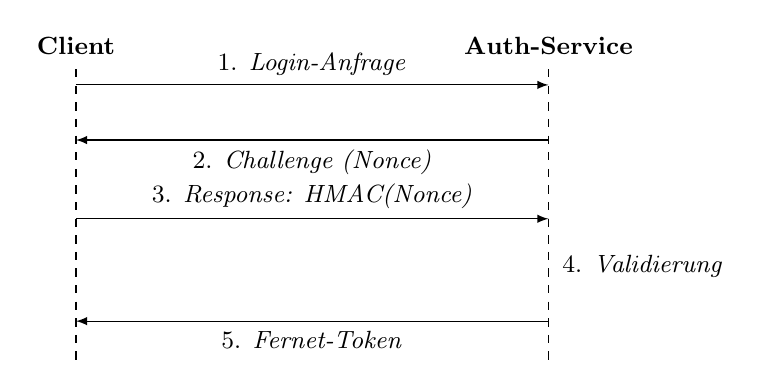
\begin{tikzpicture}[node distance=1.4cm, >=latex, every node/.style={font=\small}]
  \node (client) at (0,0) {\textbf{Client}};
  \node (server) at (6,0) {\textbf{Auth-Service}};

  % vertikale gestrichelte Linien
  \draw[dashed] (0,-0.3) -- (0,-4);
  \draw[dashed] (6,-0.3) -- (6,-4);

  % Nachrichten
  \draw[->] (0,-0.5) -- (6,-0.5) node[midway, above] {1. \textit{Login-Anfrage}};
  \draw[->] (6,-1.2) -- (0,-1.2) node[midway, below] {2. \textit{Challenge (Nonce)}};
  \draw[->] (0,-2.2) -- (6,-2.2) node[midway, above] {3. \textit{Response: HMAC(Nonce)}};
  \node at (7.2,-2.8) {4. \textit{Validierung}};
  \draw[->] (6,-3.5) -- (0,-3.5) node[midway, below] {5. \textit{Fernet-Token}};
\end{tikzpicture}
\caption{Challenge-Response-Authentifizierung mit Pre-Shared Key und Fernet-Token.}
\label{fig:auth-flow}
\end{figure}

Tokenisierung und Verwendung des Fernet-Tokens: Nach erfolgreich bestandener Chal\-lenge-Res\-ponse möchte der Server dem Client eine Art \glqq Ticket\grqq{} ausstellen, das für nachfolgende Anfragen genutzt werden kann, damit der Client nicht bei jeder Kommunikation erneut eine Challenge-Response durchführen muss. Hier kommen Tokens ins Spiel. Ein \textit{Token} ist im Wesentlichen ein Datenelement, das die erfolgte Authentifizierung repräsentiert und vom Client bei weiteren Requests mitgeschickt werden kann (\glqq bearer token\grqq{} Prinzip). Im Auth-Service wird ein solcher Token nach der Authentifizierung generiert und dem Client übermittelt (Schritt 5 in Abb.~\ref{fig:auth-flow}).

Wichtig ist, dass dieser Token sicher gestaltet ist – andernfalls könnte ein Angreifer ihn abfangen und unberechtigt benutzen (\textit{Token Hijacking}). Durch die Verwendung von Fernet stellt der Auth-Service sicher, dass der Token verschlüsselt und signiert ist. Konkret kann der Server z.B. eine Token-Payload erstellen, die folgende Informationen enthält: die Client-ID oder Kennung, ggf. Autorisierungsinformationen (Rollen/Rechte) und einen Zeitstempel bzw. Gültigkeitsdauer. Diese Payload wird dann mit dem Fernet-Schlüssel des Servers verschlüsselt, wodurch der Token entsteht. Da nur der Server den Fernet-Schlüssel besitzt, kann auch nur er den Token später wieder entschlüsseln und validieren. Selbst der Client kennt den Inhalt des Tokens nicht (es sei denn, man gibt absichtlich gewisse Felder in Klartext, was hier nicht der Fall ist).

Beim Erhalt eines Tokens speichert der Client diesen meist lokal (z.B. im Speicher oder in einem sicheren Element) und fügt ihn bei künftigen API-Aufrufen an den Auth-Service oder andere geschützte Dienste in der Kommunikationsarchitektur hinzu (oft als Teil eines Headers oder Nachricht, analog zu einem Session-Cookie). Der Server seinerseits kann eingehende Tokens überprüfen: Er entschlüsselt mit dem Fernet-Key die Payload und prüft die Gültigkeit. Dabei wird automatisch die Integrität via HMAC im Fernet gewährleistet – ist der Token manipuliert oder von einem Dritten erzeugt worden, schlägt die HMAC-Prüfung fehl und der Token wird verworfen. Zusätzlich kann der Server den Timestamp im Token ansehen und beurteilen, ob der Token noch innerhalb der erlaubten Lebensdauer liegt. Ist der Token abgelaufen, fordert der Server vom Client eine neue Authentifizierung (Challenge-Response) oder verweigert die Anfrage.
Das Zusammenspiel dieser Komponenten schafft einen robusten Authentifizierungsmechanismus:
\begin{enumerate}
    \item Der PSK liefert ein geteiltes Geheimnis als Vertrauensbasis.
    \item Die Challenge-Response-Interaktion mit HMAC beweist die Kenntnis des PSK ohne ihn preiszugeben, schützt gegen Replay und ermöglicht einmalige Authentifizierungsvorgänge.
    \item Der Fernet-verschlüsselte Token fungiert als kurzfristiger Authentifizierungsnachweis, der vom Client für wiederholte Zugriffe verwendet werden kann, ohne jedes Mal den PSK bemühen zu müssen.
\end{enumerate}


Ein großer Vorteil dieser Tokenisierung ist die Entkopplung der weiteren Kommunikation vom ursprünglichen geheimen Schlüssel. Nach der Ausstellung des Tokens muss der Client den PSK für die Gültigkeitsdauer des Tokens nicht erneut verwenden oder preisgeben. Selbst wenn ein Token kompromittiert würde (etwa durch Diebstahl), würde das zugrunde liegende PSK dadurch nicht unmittelbar bekannt. Allerdings könnte ein gestohlener gültiger Token von einem Angreifer verwendet werden (\textit{Replay Attack} mit Token). Daher ist es essenziell, die Tokens ausreichend kurzlebig zu machen und die Übertragung derselben z.B. durch Transportverschlüsselung (TLS) zu schützen.
In summe ermöglicht die Kombination aus Challenge-Response und Token eine effiziente Authentifizierung: Der rechenintensivere Teil (HMAC-Berechnung) und ein Roundtrip erfolgen nur bei der Anmeldung, während für jede weitere Anfrage der Token als Authentifizierungsbeweis dient. Der Auth-Service kann damit gegenüber nachgelagerten Diensten oder bei späteren Verbindungen schnell die Identität des Clients prüfen, indem er den Token entschlüsselt, ohne erneut eine Nutzer-Eingabe oder ein komplexes Handshake-Protokoll zu durchlaufen. Dieses Muster findet sich in vielen Systemen wieder – man denke etwa an Web-Logins, bei denen nach einmaliger Passworteingabe ein Session-Cookie ausgestellt wird.

Abschließend sei erwähnt, dass Pre-Shared-Keys und symmetrische Tokens vor allem in Szenarien zum Einsatz kommen, wo eine Ende-zu-Ende-Vertrauensstellung zwischen genau zwei Parteien besteht (hier: Gerät und Auth-Service) und die Verwaltungsaufwände für PSKs tragbar sind. In großen verteilten Systemen könnte man alternativ auch Public-Key-Verfahren einsetzen (z.B. Client-Zertifikate und JWTs mit digitaler Signatur), die andere Vor- und Nachteile bieten. Für die Zwecke des betrachteten Auth-Service – vermutlich die Absicherung einer beschränkten Anzahl bekannter Devices – liefert die beschriebene Kombination jedoch einen gut geeigneten Kompromiss aus Sicherheit und Einfachheit. Alle verwendeten Bausteine (HMAC, Fernet/AES, Challenge-Response) gelten als kryptographisch solide. Somit bilden sie eine zuverlässige Grundlage, um im Auth-Service Vertraulichkeit, Integrität und Authentifizierung sicherzustellen und gegen gängige Angriffe (Abhören, Manipulation, Replay) gewappnet zu sein.

